%%%%%%%%%%%%%%%%%%%%%%%%%%%%%%%%%%%%%%%%%%%%%%%%%%%%%%%%%%
%% HEIG-VD / institut REDS
%%
%% Modèle Latex pour laboratoire
%%
%% Fichiers à changer :
%%            - constantes.tex
%%            - Tous les fichiers du corps du rapport
%%
%% Auteur : MIM
%% Date   : 27.09.2017
%%%%%%%%%%%%%%%%%%%%%%%%%%%%%%%%%%%%%%%%%%%%%%%%%%%%%%%%%%
%% Modification: EMI, 21.03.2019 adaptation pour IFS
%%%%%%%%%%%%%%%%%%%%%%%%%%%%%%%%%%%%%%%%%%%%%%%%%%%%%%%%%%
%% MEMO :
%% Ajouter une image :  
%% \includegraphics[scale=1]{./images/Makefile.png}\\\par
%% \captionof{figure}{Makefile}
%%
%% Ajouter du code : 
%%\begin{lstlisting}[language=C]
%%  <code>
%%\end{lstlisting}
%%
%% si des annexes sont nécessaires ajouter :
%% \section{Annexes}
%%
%% Changement de notation en lettre :
%% \appendix
%% 
%% insertion d'une nouvelle page
%% \newpage
%% 
%% Ajouter un fichier latec dans le fichier courant
%% \input{Chapitres/cdc.tex}
%%
%%
%%
%%
%%

% Paramétrage du papier utilisé
\documentclass[a4paper,12pt,oneside]{article}

% Ne pas toucher, nécessaire à la mise en forme
\usepackage[utf8x]{inputenc}
\usepackage[T1]{fontenc} % Nouvelle norme pour codage des caractères
\usepackage{lmodern} % Nouvelle forme de la fonte ComputerModern
\usepackage[frenchb]{babel} % Règles typographiques françaises, césures
\usepackage{graphicx} % Insertion images
\usepackage{epstopdf} % Convertir les images eps vers pdf
\epstopdfsetup{outdir=./Images/converted_to_pdf/} % Dossier de sortie des images converties
\pagenumbering{arabic}
\usepackage[top=3cm, bottom=3cm, left=3cm, right=3cm, showframe=false]{geometry}
\usepackage{amsmath}
\usepackage{hyperref}
\usepackage{float}
\usepackage{pdfpages}
\usepackage{color}
\usepackage{caption}
\usepackage{subcaption}
\usepackage[framed,numbered,autolinebreaks]{lib/mcode}

% fichier avec les constantes (à adapter pour les étudiants)
%%%%%%%  Constantes (à changer) %%%%%%%%


\newcommand{\nomAuteur}{Pierrick Muller}

\newcommand{\titre}{<Nom Rapport>}

\newcommand{\nbrlabo}{<Num rapport>} % numéro de laboratoire

\newcommand{\prof}{<prof branche>}

\newcommand{\assistant}{<assistant branche>}

\newcommand{\classe}{<Classe>}

\newcommand{\departement}{Technologies de l'Information et de la Communication (TIC)}

\newcommand{\cours}{<Cours>}


% Entête et pieds de page (A ADAPTER)
\pagestyle{empty}
\usepackage{fancyhdr}
\setlength{\headheight}{27.06pt}
\pagestyle{fancy}
% Entête :
\renewcommand{\headrulewidth}{1pt}
\fancyhead[L]{Labo\nbrlabo: \titre}
\fancyhead[R]{Rapport de laboratoire}
% Pied de page
\fancyfoot{} % clear all footer fields
\renewcommand{\footrulewidth}{1pt}
\fancyfoot[R]{Page \thepage}
\fancyfoot[L]{HEIG-VD | \nomAuteur }

% debut du corps du rapport
\begin{document}
	% première page
	%%%%%%%%%%%%%%%%%%%%%%%%%%%%%%%%%%%%%%%%%%%%%%%%%%%%%%%%
% Ce document ne doit pas être modifié
% Il faut modifier les informations depuis le fichier
% constantes.tex
%%%%%%%%%%%%%%%%%%%%%%%%%%%%%%%%%%%%%%%%%%%%%%%%%%%%%%%%



\begin{center}

\includegraphics[height=2cm]{./images/logo_heig.pdf}
\hfill 
\includegraphics[height=2cm]{./images/logo_hesso.pdf}
\end{center}

\vfill

\begin{center}
	\Large Laboratoire \nbrlabo:\\
	\huge \titre \\
\end{center}


\begin{center}
	\begin{tabular}{l l}
		Département:          & \departement\\
		Unité d'enseignement: & \cours\\
	\end{tabular}
\end{center}


\vfill

%\begin{center}
%	\includegraphics{Images/it.png}
%\end{center}

\vfill

\begin{tabular}{l l}
	\Large	Auteurs:   			  & \Large \nomAuteur\\
	Professeur:           & \prof\\
	Assistant:			  & \assistant\\
	Classe:               & \classe\\
	Date:                 & \today\\
\end{tabular}

\vfill

\begin{center}

\includegraphics[height=1.5cm]{./images/logo_reds.pdf}
\end{center}
	% enlève le numero sur la premiere page
	\thispagestyle{empty}
	\setcounter{page}{1}
	\newpage

	% ici débute le corps du rapport
	% changer les sections au cas par cas afin de vous adapter au maximum aux critères
	%\section{Introduction}
	%\section{Analyse et conception}
	%\section{Réalisation et implémentation}
	%\section{Simulation}
	%\section{Conclusion}
	% les méthodologies présentée ci-dessus est une bonne approche pour les petits projets qui ne demandent pas beaucoup de documentation mais n'est pas adaptée à des gros projets où plusieurs personnes vont rédiger de la documentation (Utilisation de git)
	% En modifiant les documents depuis deux endroits différents, si vous répartissez le travail par "thème", chacun va modifier un document et à la fin il suffira de merge ensemble les changements
	\tableofcontents

	\newpage

	\section{Priorité des threads et Linux}

\par
\begin{figure}[H]
%%\centering
\begin{subfigure}{.5\textwidth}
  \centering
  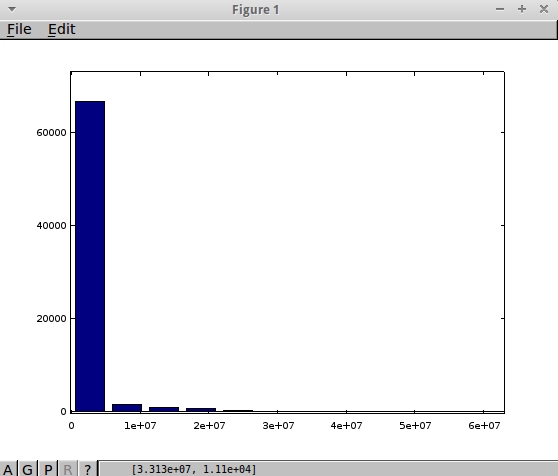
\includegraphics[width=.9\linewidth]{./img/part1_octave.png}
  \caption*{Histogramme}

\end{subfigure}%
\begin{subfigure}{.5\textwidth}
  \centering
  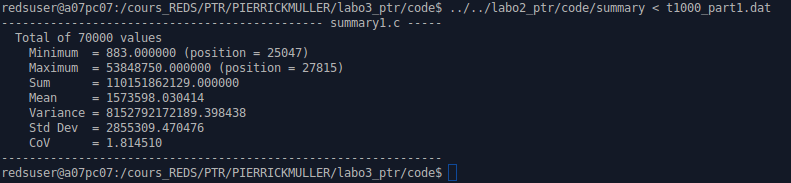
\includegraphics[width=.9\linewidth]{./img/part1_summary.png}
  \caption*{Sommaire}

\end{subfigure}
\caption{Résultat tests avec le programme dohell sur le programme "timer.c" avec un temps d'attente de $1ms$, 70000 mesures }

\end{figure}

	\section{Analyse et conception}


\begin{itemize}
\item item1
\item item2
\item item3
\end{itemize}

	\section{Réalisation et implémentation}

\subsection*{sous-titre de section:}

	%\section{Simulation / Problèmes majeurs rencontrés}

	%\section{Conclusion}


	%Section pour la signature
	\section{Signatures}

    Yverdon-les-Bains le \today \\
    \begin{center}
      \nomAuteur
    \end{center}

	\listoffigures
	% si des annexes sont nécessaires ajouter :
	% \section{Annexes}
	% Changement de notation en lettre :
	%\appendix
	% insertion d'une nouvelle page
	%\newpage
	% Ajouter un fichier latec dans le fichier courant
	%\input{Chapitres/cdc.tex}



%Fin du document
\end{document}
